\documentclass[a4paper,11pt]{report}
\usepackage[latin1]{inputenc}
\usepackage[english]{babel}
\usepackage{graphicx} 
\usepackage{pdfpages}
\usepackage{fancyvrb}
\usepackage{tabularx}
%\usepackage{pifonts}
%\newcommand{\tick}{\ding{52}}
\newcommand{\tick}{$\times$}

\usepackage{amsmath}
\newcommand{\argmax}{\operatornamewithlimits{argmax}}

\usepackage{cite}
\usepackage{url}
\bibliographystyle{unsrt}

\graphicspath{{images/}}
\begin{document}

\begin{titlepage}
\begin{center}

\includegraphics[width=5cm]{EURECOM_logo_quadri}
\\[3cm]
\textbf{\Huge{TBD}}
\\[2cm]
\textbf{\textsc{\LARGE{Semester Project Report}}}
\\[0.5cm]
\LARGE{Luca Venturini}
\\
\large{Spring 2013}
\\[8cm]
\columnsep3cm
\begin{tabular}{p{8cm} p{8.5cm}}
\small{\textbf{Supervisors:}\newline
Giuseppe Rizzo} \newline
Rapha\"el Troncy
&
\small{\textbf{EURECOM\newline Multimedia Department}}
\end{tabular}
\end{center}
\end{titlepage}

 \tableofcontents

\chapter{Introduction}
\label{sec:intro}
Natural Language Recognition studies how to allow a machine to understand and possibly interact with an human being by means of the word, without any other kind of interactions between the two. A sign, such as a word, is formed by a signifier and a signified; only the former, the word itself, is accessible to the machine, while the latter is something meaningful only for men. However, machines can store and elaborate information correlated to signifiers, as well as all the linkages between them, without the need to understand their meaning. In other words, a machine is useful whenever it can shorten the path linking two pieces of information and show to the man the final linkage, saving the time to go through all the path. Hence a machine can state the average life span for English monarchs, simply going through a knowledge base of historical figures and retrieving values for "age at death", without knowing the meaning of life or death (which would be problematic for men as well).

Usually a machine is able to work on structured data, i.e. where the pairs field-value and the relations are explicit, as in the previous example. The main goal of Natural Language Recognition is to retrieve information from unstructured data, as a news article or a free-text form. In the context of Web today, we see Petabytes of unstructured data "in the wild", and search engines which would like to index and understand some of the content enclosed in these pages; an effort to reach this result has been led by the promoters of Semantic Web, which attempts to have an uniform semantics over web pages dealing with the same topics, by means of tags (i.e. structured data "hidden" in the code of the page). However, too much unstructured information still exists to be manually structured by man.

\section{Named Entities}
A Named Entity is an entity which has a rigid designator, like a name (C.S. Lewis) or a number (year 1789). The definition of "rigid" can be loosened, depending on the task; sometimes money and time expressions are considered Named Entities as well, even in the cases they do not define uniquely a value (as in "at noon", when we don't know the 12 o'clock of which day we are talking about). Entities are named and unique even if they are not so in the text where they appear: in the sentence "The Queen died in 1603", "The Queen" is a designator for Queen Elizabeth I even if her name is not manifestly written, so a Named Entity Extractor should be defined to include such cases in the Named Entities.

Named Entity Extraction, also known as Named Entity Recognition (NER), and Named Entity Linking (NEL) are subtasks of Information Extraction. In NER, we want to extract all the entities cited in a document and recognize their type (such as Person or Organization). In NEL, we want to link a Named Entity (referred by the name by which it appears in the document and its position) to a node in a Knowledge Base (KB), e.g. Wikipedia. Together with Slot Filling, which allows to fill the values in the KB nodes from their unstructured description, this tasks form the bigger task of automatically building a Knowledge Base from raw data.

\section{The problem}
Named Entity Recognition needs a first phase of training: a big training set is needed to reach good results, data needs to be collected from various sources and labelled. The very first extractors were trained on articles from newspapers; but performances on different type of contexts (such as Web fora, narrative, email messages...) are much worse than on documents from the same type of source, or maybe the same newspaper.

The challenge here is to study how extractors can adapt to different contexts or corpora and how well they can react to the adaptation. In the next section, we will provide an insight on a NER system designed at Stanford, in order to give an understanding on how such training could be approached and what does it mean having a trained model. Next, we will look at TAC KBP evaluation campaign, where other Natural Language systems are compared and new trends for research in the field are proposed; we will focus particularly on NEL systems and their global performances, to have an idea on the evaluation method. Finally, we will present our web service, an interface to Stanford NER which allows an user to train it from own datasets.
%The final goal is to integrate it in a system which provides a single interface to many NER systems, NERD.

\chapter{State of the art}

\section{Conditional Random Fields}
\label{sec:crfs}
Conditional Random Fields (CRFs) were introduced by Lafferty, McCallum and Pereira in 2001\cite{lafferty2001conditional} as a probabilistic model to segment and label sequence data. Considering our Named Entity Recognition task as a subtask of the labelling problem, we can define a log-linear model
$$
p(\overline{y} \mid \overline{x}; w) = \frac{1}{Z(\overline{x}, w)}\exp\sum\limits_j w_jF_j(\overline{x}, \overline{y})
$$
where $\overline{x}$ and $\overline{y}$ are our training sequence and the respective label sequence, $w_j$ are real-valued weights for feature functions $F_j$ and $Z$ is a partition function, defined as
$$
Z(\overline{x}, w) = \sum\limits_{\overline{y}}\exp\sum\limits_j w_jF_j(\overline{x}, \overline{y})
$$
A model can contain hundreds of thousands of different feature functions, which are computed over a single word, its position in the sentence, its labelling and possibly all the surrounding context (the whole $\overline{x}$ and $\overline{y}$). As example, consider the word "A.C.M.E.": its punctuation and the capitalization are two features strongly suggesting we are talking about an organization.

Hence, training $w$ corresponds to the Maximum Likelihood Estimation of the parameters of our model, that is to say
$$
\hat{w} = \argmax_w p(\overline{y} \mid \overline{x}; w)
$$
Inference and decoding of $\overline{y}$ from a new sample $\overline{x}$ (i.e., labelling a document), will therefore correspond to
$$
\hat{y} = \argmax_y p(y \mid \overline{x}; \hat{w})
$$
There exist lots of methods to solve these two maximization problems in literature, and algorithms applied to the context of CRFs are still an interesting research field. Special training algorithms have been proposed, namely stochastic gradient ascent and derivations of Collins perceptron \cite{elkan2008log}.

\section{Stanford NER}
\label{sec:StfdNER}
Stanford NER \cite{finkel2005incorporating} is a Java implementation of Conditional Random Fields for Named Entity Recognition, coupled with good feature extractors. The software provides interfaces to access the main utilities by command line and APIs to control the classifier (also known as CRFClassifier, to disambiguate from other tools developed by the same university based on Hidden Markov Models).

The main difficulty approaching Stanford NER is the lack of documentation; little tutorials exist on using it by command line, but the only hints on APIs functioning are given by a couple of demos and the sourcecode itself.

The software allows to train the classifier from own data; as we have seen in Section \ref{sec:crfs}, we need some training data, i.e. a dataset of labelled documents. The input format makes the token-label pairs explicit by listing a token per line, as in the following example (where the character O stands for "Other"):


\begin{table}[h]
\begin{center}
\begin{tabular}{ll}
Sixteen &	O\\
years	& O\\
had	&O\\
Miss	&PERS\\
Taylor	&PERS\\
been	&O\\
in	&O\\
Mr.	&PERS\\
Woodhouse	&PERS\\
's	&O\\
family	&O\\

\end{tabular}
\end{center}
\caption{Input format for training datasets}
\label{tab:inputfmt}
\end{table}


Once a model for the classifier is trained, it cannot be modified; however, since the training is deterministic, it is still possible to create new instances of the classifier from scratch. Trained classifiers are serialized and compressed into an archive storing the necessary parameters to reload it.

Together with the library, Stanford provides already some good serialized classifiers, trained on 3 (Location, Person, Organization), 4 (Location, Person, Organization, Misc) and 7 Entity Types (Time, Location, Organization, Person, Money, Percent, Date), trained on CoNLL 2003 and MUC English training data. A typical use case sees the user loading these models from memory and elaborate some document, skipping the training part.

\chapter{TAC KBP evaluation campaign}
Text Analysis Conference (TAC) was born in 2009 to lead the research in Natural Language Processing, by means of the proposal of several tracks of study and a common definition of objectives, challenges and evaluation criteria. This effort, shared by many universities and research teams in the world, aims both to bring new solutions and to propose new challenges to the community. The track we are particularly interested in, for the tight relationship with the work on Named Entities, is Knowledge Base Population (KBP).

KBP task is actually made of many subtasks: in the following sections, we will specifically focus on two of them, Slot Filling and Entity Linking task, that we already introduced in \S \ref{sec:intro}. The discussion of this topic is in any way meant to be exhaustive, but we would like to give here an interesting introspection on the problems, the solutions proposed and the evaluation of the results.
%TODO insert space

Task supervisors define the goals, the evaluation criteria and the format for the queries and provide the participants of a 2008 Wikipedia snapshot as referral Knowledge Base and some corpora of texts to train the systems. Other useful instruments are provided as well, such as mappings for Wikipedia infobox fields, which sometimes have non-unique identifiers.

Task definitions can be found at %TODO cite.

%TODO better specify the general approach of the "shared task"

\section{Slot Filling task}
Slot filling task aims to populate the fields of a structured form with data coming from unstructured knowledge. The typical scenario is the population of a Knowledge Base, such as Wikipedia: in this case, the structured form is Wikipedia infobox, whose fields vary depending on the type of the entity in object, and the unstructured knowledge is the text of the page (the description, in plain English).
We may want, for example, to extract some missing values for movie director Steven Spielberg, like the name of his spouse or children, directly from the text, or from a corpus of news articles. Obviously, a Slot Filler should also consider the case where such values are not pertinent, and the slot should not be filled (e.g., there are no children for a given person).

\begin{table}
\begin{tabularx}{\linewidth}{lXXXX}
 & 2009 & 2010 & 2011 & 2012 \\
\hline Entity types \\ 
  PER & \tick & \tick & \tick & \tick \\
  ORG & \tick & \tick & \tick & \tick \\
  GPE & \tick & & & \\
\hline Corpus & 1M articles & added 500K weblogs, more topics, more formats & added 1M newswire & added 1M webtext + 1M Spanish texts \\
\hline Tasks\\ 
 Slot Value linking & \tick & & & \\
  Surprise Slot Filling & & \tick & & \\
  Temporal Slot Filling & & & \tick & \\
  Cross-lingual Slot Filling & & & & EN + Spanish \\
  Slot filler validation (SFV) & & & & \tick \\
  Confidence scores & & & & \tick \\
  Justification & & & & \tick \\
\hline Other issues\\ 
 Closed systems & & \tick & \tick & \tick \\
 

\end{tabularx}

\caption{Comparison of the Slot Filling task definition in the years}
\label{tab:sf}
\end{table}

Table \ref{tab:sf} shows a quick summary of the task in the years. First, we can notice that the corpus for training has been always growing, adding different types of sources. Entity types for which the slot filling task was required were initially Person, Organization and Geo-Political Entity: the last mentioned has been dropped in the following editions, since information in the corpora on such entities was not enough to fill the slots (usually, news articles citing toponyms do not give details useful for a Knowledge Base, like the number of inhabitants).

The number and type of subtasks changed a lot through the years, including the following:

\begin{description}
\item[Slot value linking] This task consisted in linking the new filled slot with the appropriate entity in the KB (e.g. after having filled the value for Steven Spielberg's father, link it to the node for the right Arnold Spielberg). Since it had great overlap with the Entity Linking task, it was dismissed after the very first year.
\item[Surprise Slot Filling] The teams were required to compete on a surprise subject and submit results in 4 days. A few teams participated.
\item[Temporal Slot Filling] Together with the filling values, participating systems are required to provide the date when this value has been valid (e.g. for a "spouse" field, date of marriage and divorce). The task was divided in full filling (i.e. finding the values and provide the dates) and diagnostic filling (i.e. state, given the slot filling value, in which dates this value was valid). This task will be retried in 2013.
\item[Cross-Lingual slot filling] Spanish language was added to the task.
\item[Slot Filler Validation] The input of such a system is the output of other Slot Filling systems; the output, for each of them, is just whether they are correct or incorrect.
\item[Confidence Scores] For each value to fill a slot, a confidence score between 0.0 and 1.0 is given. This score states how sure the system is of the choice; having different possible values for a given slot, the sum of all the confidence scores for those values is 1.
\item[Justification] Together with the answer, a justification is given, in the form of a mention to the document id and offset in the page where such a justification can be found. For instance, a justification can be "From 1985 to 1989 Spielberg was married to actress Amy Irving".
\item[Sentiment] In 2013, systems will optionally be required to state whether a value for a slot is given with a positive or negative sentiment (or neutral).
\end{description}

After the first year, participants were also asked to submit at least one run with closed systems, that is without access to web knowledge bases or search engines (e.g. Google).

\section{Entity Linking task}
We will approach the problem of Entity Linking first with an example.

Suppose we have the following sentence:
\begin{quote}
After his death, Armstrong was described, in a statement released by the White House, as "among the greatest of American heroes - not just of his time, but of all time".
\end{quote}

After having correctly recognized the entity "Armstrong", and maybe having labelled it as a person, we would like to disambiguate it. Which Armstrong is it referring to? First, we should start thinking of all the Armstrongs we might know: Louis the jazzer, Lance the cyclist, Neil the astronaut...then, among the ones we have thought of, we should individuate who is dead and American. If there is still some ambiguity, we should eventually begin to reason on who is most probable to be named as "hero" by the White House, or find this sentence in an useful context.\footnote{This sentence referred to Neil Armstrong (1930 - 2012).}

This example shows some of the problems occurring with Entity Linking, which can be defined as the problem of linking a Named Entity to the node in a knowledge base which it refers to. The challenge here is to face different sources of ambiguity, in order to link the Named Entity to the correct KB node: we have a one-to-many ambiguity, as in the example above, where the same string can refer to different nodes, but we have a many-to-one ambiguity as well, since the same entity in a KB node could be designated in different ways, by short names, by the initials, by just the first name or the surname, or maybe for a misspelling or transliteration. For instance, Louis Armstrong's full name was Louis Daniel Armstrong, but he was often nicknamed Satchmo (for satchel-mouth) or Pops.

In Table \ref{tab:el} we see how the task has been developed through the years. Entity types, differently from Slot Filling task, have not changed. Corpus provided is the same as the one for Slot Filling, plus some additions for Cross-Lingual task. The task requires answers to be either the identifier of the KB node linked to the Named Entity in the query or NIL, if no nodes in the KB exist for it.
Some subtasks were added in the years, but they are not mandatory.
\begin{description}
\item[Optional task] The goal of this subtask is to submit a system which does not make use of the description in the Wikipedia page, but only the fields in the infobox. This task was introduced because such systems can be easily applied to knowledge bases containing only structured data (which is often the case).
\item[NIL Clustering] The subtask requires, for all NILs found, to cluster the ones which refer to the same entity. Together with Slot Filling this can form the basis for automatic insertion of new nodes in the KB.
\item[Cross-Lingual task] The system should link entities found in another language (Chinese) text to English KB.
\end{description}

\begin{table}
\begin{tabularx}{\linewidth}{lXXXX}
 & 2009 & 2010 & 2011 & 2012 \\
\hline Entity types \\ 
  PER & \tick & \tick & \tick & \tick \\
  ORG & \tick & \tick & \tick & \tick \\
  GPE & \tick & \tick & \tick & \tick \\
\hline Corpus & 1M articles & added 500K weblogs, more topics, more formats & added 1M newswire + 1M Chinese texts & added 1M webtext + 1M Chinese articles + 800K web texts\\
\hline Tasks\\ 
Optional Task & & \tick & \tick & \tick \\
NIL Clustering & & & \tick & \tick \\
Cross-Lingual  & & & \tick & \tick \\
 
 

\end{tabularx}

\caption{Comparison of the Entity Linking task definition in the years}
\label{tab:el}
\end{table}

\subsection{General approach to EL system design}
Studying the EL systems proposed to TAC we can individuate some general trends in their structure, as well as some common techniques which seem reasonable and intuitive.
The core of all the systems is made of two critical phases: Candidate Generation and Candidate Ranking. This is indeed a natural way to proceed, and reflects the same approach we adopted in our previous example: to think of all possible entities with the given name and to figure out which of them is the most probable to be.

Candidate Generation phase is usually based on a research, on the KB, of all the terms of the query; we usually also see some techniques to enlarge the set of candidates with less probable entities, in order to be sure the exact one, if it exists, is in the set. Here the most intuitive techniques, like a search in the title, perform well enough.
Given the set of candidates, Candidate Ranking aims to assign a likelihood score, and choose whether the first candidate in the ranking is likely enough to be the answer, or if we don't have any link with the KB instead (NIL answer).

We can see the two core phases in the general architecture in Figure \ref{fig:el_arch}. As we can notice, Candidate Generation is supported by some preprocessing phases, as Query Expansion, whose goal is to improve the query (expanding acronyms or adjusting misspellings) or Mention Collaborators, used in systems like UIUC's Wikification (Section \ref{sec:uiuc}). %TODO reference
 Finally, and optionally, in the case the answer is NIL NIL Clustering is executed.
 
\begin{figure}[htbp] 
\centering
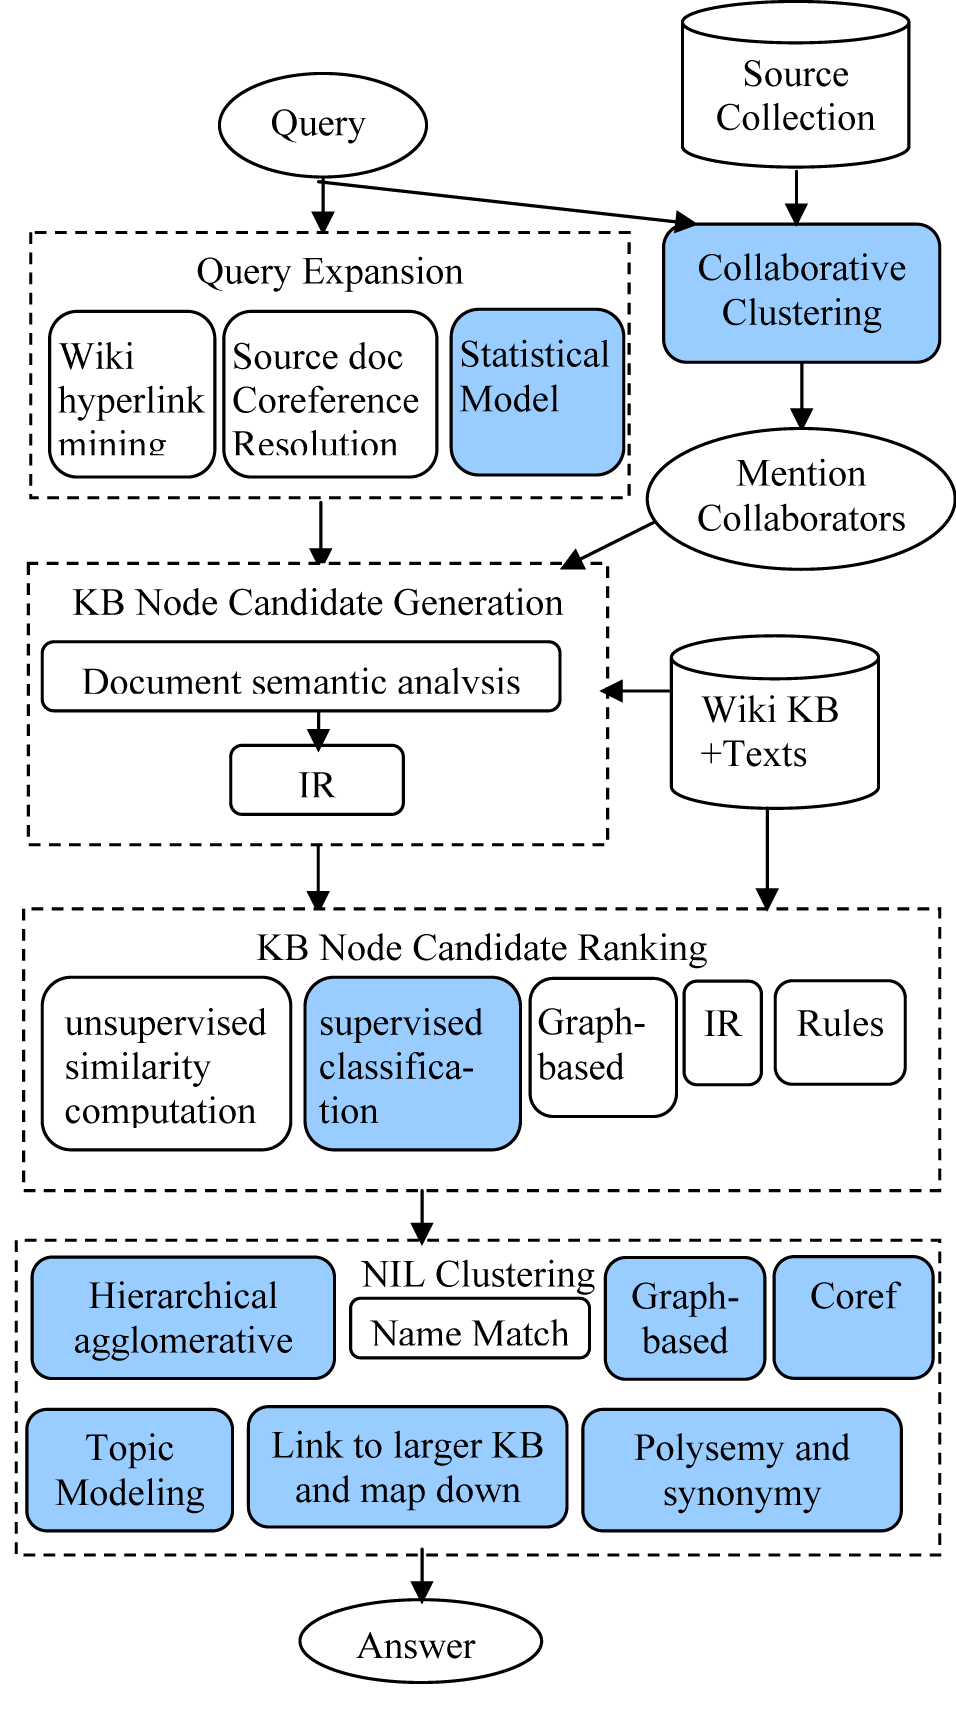
\includegraphics[]{el_architecture}
\caption{General Entity Linking system architecture}
\label{fig:el_arch}
\end{figure}


\chapter{Building a framework for NER adaptation}

%introduction and example of use
In this chapter, we will see how we developed a NER framework based on Stanford NER (Section \ref{sec:StfdNER}). The system provides a web interface which allows an user to train the classifier loading own datasets, and to use it on own documents. %TODO check this sentence
The web service is fully compliant to REST principles, %TODO footnote?
hence APIs are of easy access from a client implementing HTTP methods. 

\section{Profiling Stanford NER}
To design a service aimed to several users, able to manage different requests at the same time is not a trivial task. Performances of a NER system greatly vary accordingly to the input size (both for training and extraction) and can take the waiting time for the users over limits of bearability. Before approaching the whole design, we investigated on the bottlenecks of Stanford NER system, in order to understand which phases would have taken the biggest part in response time.

Tools used to profile Java code were the ones integrated in VisualVM \footnote{\url{http://visualvm.java.net}}.

\begin{figure}[htbp] 
\centering
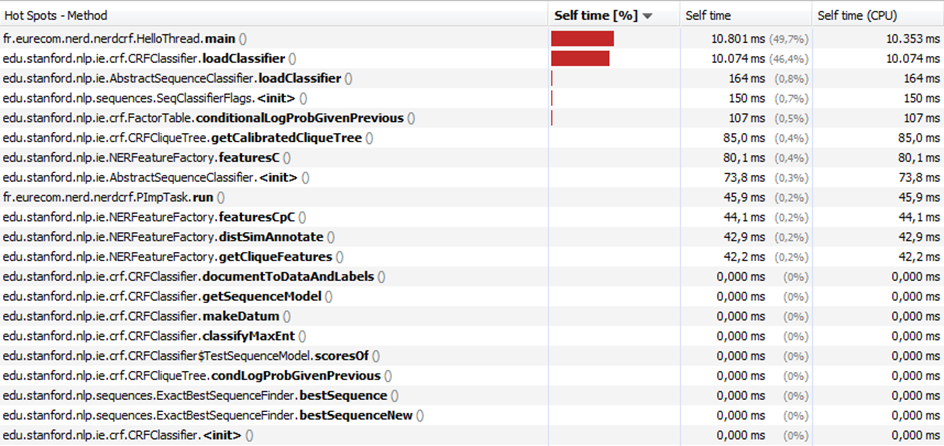
\includegraphics[width=\textwidth]{functions}
\caption{CPU usage per function call (small text)}
\label{fig:profile1}
\end{figure}

\begin{figure}[htbp] 
\centering
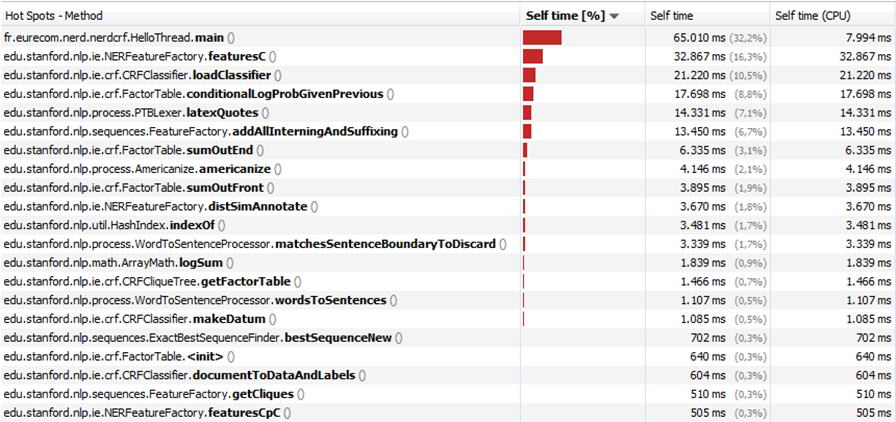
\includegraphics[width=\textwidth]{functions2}
\caption{CPU usage per function call (large text)}
\label{fig:profile2}
\end{figure}

We executed tests on a small text (the main content of a Wikipedia page)(Figure \ref{fig:profile1}) and on a bigger one, Jane Austen's Pride and Prejudice (Figure \ref{fig:profile2}).
As we can see in Figure \ref{fig:profile1}, the greatest part of the execution time is spent loading the model of the classifier from memory. As input size grows, the initial loading takes less percentage of the time, but it is still a remarkable load. In Figure \ref{fig:profile2} we notice also a second function taking a good slice of CPU time, \texttt{featuresC()}: this function is indeed in charge of tokenizing the text.

This data clearly show the need for avoiding unnecessary loads from disk: frequently used models should be kept in cache whenever possible, taking care of the hardware limits, since models can have great space requirements.

\section{Schema of resources}
%introduction to rest principles
Representational State Transfer (REST) is a software architecture style defined in 2000 by Roy Fielding and emerged as predominant design model for web APIs. %TODO cite Fielding?
In REST, client-server communication is based on the transfer of resource representations; therefore, we need to define what these resources are, how we identify them (URIs), by which HTTP method we can interact with them (GET, POST, PUT, DELETE) and which representation do we want for them.
Our system accepts requests for representations in XML or JSON.
Resources are the following (URI are given with relative path):
\subsection*{Documents}
The main collection for documents to be elaborated. Its URI is \texttt{/documents}.
Methods accepted:

\begin{description}
\item{POST} Create a new document, whose text is specified in the mandatory field \texttt{text}.
\end{description}

\subsection*{Document}
The document to be elaborated, i.e. whose entities we want to extract. Its URI is \texttt{/documents/\{doc\_id\}}.
Methods accepted:

\begin{description}
\item{GET} Get the representation for the document.
\end{description}

\subsection*{Annotations}
The main collection for results from extraction. Its URI is \texttt{/annotations}.
Methods accepted:
\begin{description}
\item{POST} Create a new annotation for document specified in field \texttt{id}, with the model specified in field \texttt{model} (optional). If model is not specified, the default one will be used.
\end{description}

\subsection*{Annotation}
The result from an extraction, a list of all entities recognized in the text. Its URI is \texttt{/annotations/\{ann\_id\}}. Methods accepted:
\begin{description}
\item{GET} Get the representation for the list of entity-label pairs.
\end{description}

\subsection*{Models}
The main collections for models. Its URI is \texttt{/models}. Methods accepted:
\begin{description}
\item{POST} Create a new model.
\end{description}

\subsection*{Model}
A model for Stanford classifier, i.e. a collection of training datasets. Its URI is \texttt{/models/\{mod\_id\}}. Methods accepted:
\begin{description}
\item{POST} Create a new training dataset for the model, from a file posted with content-type multipart/form-data, in CoNLL format (as in Table \ref{tab:inputfmt}). 
\end{description}

%TODO get for the training files?

\section{A sample use case}
%APIs
In the following scenario, an user tries the framework by submitting a document to the classifier with the default model; then, he repeats the experiment with a model self-trained, on a training set based on the first chapter of Jane Austen's Emma, where Named Entities of type Person are labelled.

The client used is \texttt{curl}\footnote{\url{http://curl.haxx.se}}.

\cleardoublepage
\addcontentsline{toc}{chapter}{Bibliography}
\bibliography{biblio}
\nocite{*}


\end{document}
